\documentclass{exam}

\usepackage{amsmath,amssymb,amsthm}

\usepackage{pgf,tikz}\usepackage{mathrsfs}\usetikzlibrary{arrows}\pagestyle{empty}

\title{Math 121 - Readiness Assessment \# 4}
\date{}
%Key - D028

\begin{document}
\maketitle

\begin{questions}
\question
The point $A$ on this graph would be a:
\definecolor{qqqqff}{rgb}{0,0,1}
\definecolor{cqcqcq}{rgb}{0.7529411764705882,0.7529411764705882,0.7529411764705882}
\begin{center}
\begin{tikzpicture}[line cap=round,line join=round,>=triangle 45,x=1cm,y=1cm,scale=0.8]
\draw [color=cqcqcq,, xstep=1cm,ystep=1cm] (-2.646618050747502,-4.775447812015698) grid (3.920767959314037,4.785893584985674);
\draw[->,color=black] (-2.646618050747502,0) -- (3.920767959314037,0);
\foreach \x in {-2,-1,1,2,3}\draw[shift={(\x,0)},color=black] (0pt,2pt) -- (0pt,-2pt) node[below] {\footnotesize $\x$};
\draw[->,color=black] (0,-4.775447812015698) -- (0,4.785893584985674);
\foreach \y in {-4,-3,-2,-1,1,2,3,4}\draw[shift={(0,\y)},color=black] (2pt,0pt) -- (-2pt,0pt) node[left] {\footnotesize $\y$};
\draw[color=black] (0pt,-10pt) node[right] {\footnotesize $0$};\clip(-2.646618050747502,-4.775447812015698) rectangle (3.920767959314037,4.785893584985674);
\draw[smooth,samples=100,domain=-2.646618050747502:3.920767959314037] plot(\x,{0-((\x)-1)*((\x)-3)*((\x)+1)});
\begin{scriptsize}
\draw [fill=qqqqff] (2.151230677190442,3.0678280630934145) circle (2.5pt);
\draw[color=qqqqff] (2.2651244273657505,3.357901038680274) node {$A$};
\end{scriptsize}
\end{tikzpicture}
\end{center}
\begin{oneparchoices}
\choice Local maximum
\choice Local minimum
\choice Absolute maximum
\choice Absolute minimum
\end{oneparchoices}
\question At any point where a function is increasing, the derivative must be:
\begin{oneparchoices}\\
\choice Zero
\choice Non-existant
\choice Negative
\choice Positive
\end{oneparchoices}
\question The Extreme Value Theorem can be used to find out what information?
\begin{choices}
\choice The absolute max/min of a function, for all values.
\choice The derivative of a function
\choice Where a function is continuous.
\choice The absolute max/min of a function, on a closed interval.
\end{choices}
\question The Extreme Value Theorem has a familiar hypothesis about which kind of function it can apply to. What is that hypothesis?
\begin{choices}
\choice The function must be increasing.
\choice The function must be decreasing.
\choice The function must be continuous.
\choice The function must be differentiable.
\end{choices}
\newpage
\question A critical number of a function $f$ is a number $c$ in the domain where which of these happens?\\
\begin{choices}
\choice The function is differentiable at $c$.
\choice $f'(c) = 0$.
\choice The function is not defined at $c$.
\choice $f'(c) = 0$, or it does not exist.
\end{choices}
\question The following image is often shown with the Mean Value Theorem. What can we assume about the derivative of the function $f$ when $x=c$ and the slope of the line connecting the points where $x=a$ and $x=b$?
\begin{center}
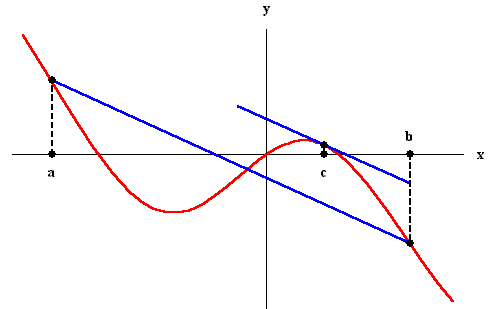
\includegraphics[width=0.6\textwidth]{Image01}
\end{center}
\begin{choices}
\choice The derivative at $x=c$ is the same as the slope of the line from $x=a$ to $x=b$.
\choice The derivative is zero when $x=c$.
\choice All values of the derivative exist between $a$ and $b$
\choice There is a local maximum when $x=c$
\end{choices}
\question What happens at a point of inflection?
\begin{choices}
\choice The graph may change from increasing to decreasing.
\choice The graph may change concavity.
\choice The function has a local maximum.
\choice The function has a local minimum.
\end{choices}
\question
Which of these would be described as an optimization problem?
\begin{choices}
\choice Find the relationship between the change in volume of a sphere and the change in it's radius.
\choice Proving a real zero of an equation exists over a certain interval.
\choice Finding the slope of the tangent line to a curve at a specific point.
\choice A business owner wanting to maximize profits and minimize costs.
\end{choices}
\question
Optimization problems always require that we find which of the following?
\begin{choices}
\choice Absolute maximum or minimum of a function.
\choice Local maximum or minimum of a function.
\choice Intervals where a function is increasing or decreasing.
\choice Intervals where a function is concave up or concave down.
\end{choices}
\question At any point where a function is decreasing, the derivative must be:
\begin{oneparchoices}\\
\choice Zero
\choice Non-existant
\choice Negative
\choice Positive
\end{oneparchoices}
\end{questions}
\end{document}